% !TEX encoding = UTF-8
% !TEX TS-program = pdflatex
% !TEX root = ../tesi.tex

%**************************************************************
\chapter{Framework Flutter e linguaggio Dart}
\label{cap:Framework Flutter e linguaggio Dart}
%**************************************************************

\intro{In questo capitolo, viene introdotto come un'applicazione mobile può essere sviluppata per poi concentrarsi su Flutter e tutte le sue componenti. Infine saranno mostrate come esempio alcune piccole applicazioni realizzate per imparare a utilizzare il framework Flutter.}\\

%**************************************************************
\section{Sviluppo applicazioni mobile}
Nel quotidiano, non solo in Italia ma in tutto il mondo, l'uso dello smartphone \cite{statistiche} è in costante aumento. \\
Mentre fino a qualche anno fa il cellulare veniva usato solo per telefonare o mandare qualche messaggio, oggi lo smartphone viene utilizzato in qualsiasi ambito: lavoro, comunicare, divertirsi, video, musica o svago. \\
Ormai nei cellulari sono presenti applicazioni per qualsiasi esigenza ed è proprio per questo che chi sviluppa applicazioni ha dovuto considerare lo sviluppo per mobile come fattore primario.\\
	\begin{figure}[htbp]	
	\centering
	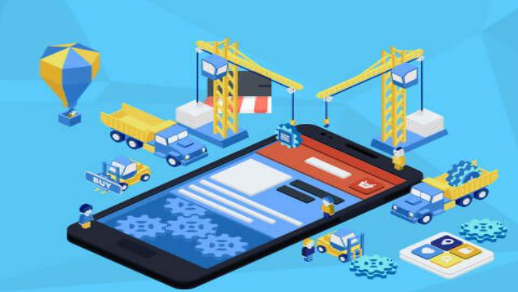
\includegraphics[width=10cm]{immagini/sviluppoapp.png}
	\caption{Sviluppo applicazioni mobile}
	\label{fig:Sviluppo applicazioni mobile}
\end{figure}
\\
Esistono quattro diversi approcci di implementazione: 
\begin{itemize}
	\item App native; 
	\item Web app; 
	\item App Ibride Web View Wrapper; 
	\item App Ibride Compile to Native.
\end{itemize}
\cite{sviluppo,differenza,apptonative}

\subsection{App native}
Il metodo nativo \cite{differenza,apptonative} da la possibilità all'applicazione di integrarsi con la parte hardware del dispositivo, sfruttando così tutte le funzionalità del sistema operativo. \\
Le app native vengono realizzate utilizzando gli strumenti di sviluppo software e la documentazione fornita dai produttori del sistema operativo per il quale si ha l'intenzione di sviluppare.\\
Questo metodo è scelto sopratutto degli sviluppatori attenti alle prestazioni e alle performance dell'applicazione.\\
I vantaggi principali di sviluppare App native sono:
\begin{itemize}
	\item Maggiore velocità, affidabilità e reattività;
	\item Accesso diretto alla parte hardware e al software installato nel device; 
	\item Notifiche dirette;
	\item Funzionamento offline.
\end{itemize}
Attualmente i sistemi operativi più utilizzati sono:
\begin{itemize}
	\item Android; 
	\item iOS; 
	\item Windows Phone.\\
\end{itemize}
\cite{sviluppo}

\subsubsection{Android}
\begin{figure}[htbp]	
	\centering
	
\includegraphics[width=1cm]{immagini/logoandroid.png}
	\caption{Logo Android}
	\label{fig:Logo Android}
\end{figure}
 Android è il sistema operativo più utilizzato e diffuso. È stato sviluppato da Google ed è stato scelto da multinazionali importanti come Samsung, Huawei e Amazon per il funzionamento dei loro dispositivi.\\
 Il linguaggio per sviluppare un'applicazione Android è Java. Negli ultimi anni è nato anche Kotlin, che è un altro linguaggio ufficiale per la progettazione di applicazioni Android più moderno, meno complesso ma performante e compatibile con l'ambiente Android quanto Java.\\
 \newpage

 \subsubsection{iOS}
 \begin{figure}[htbp]	
 	\centering
 	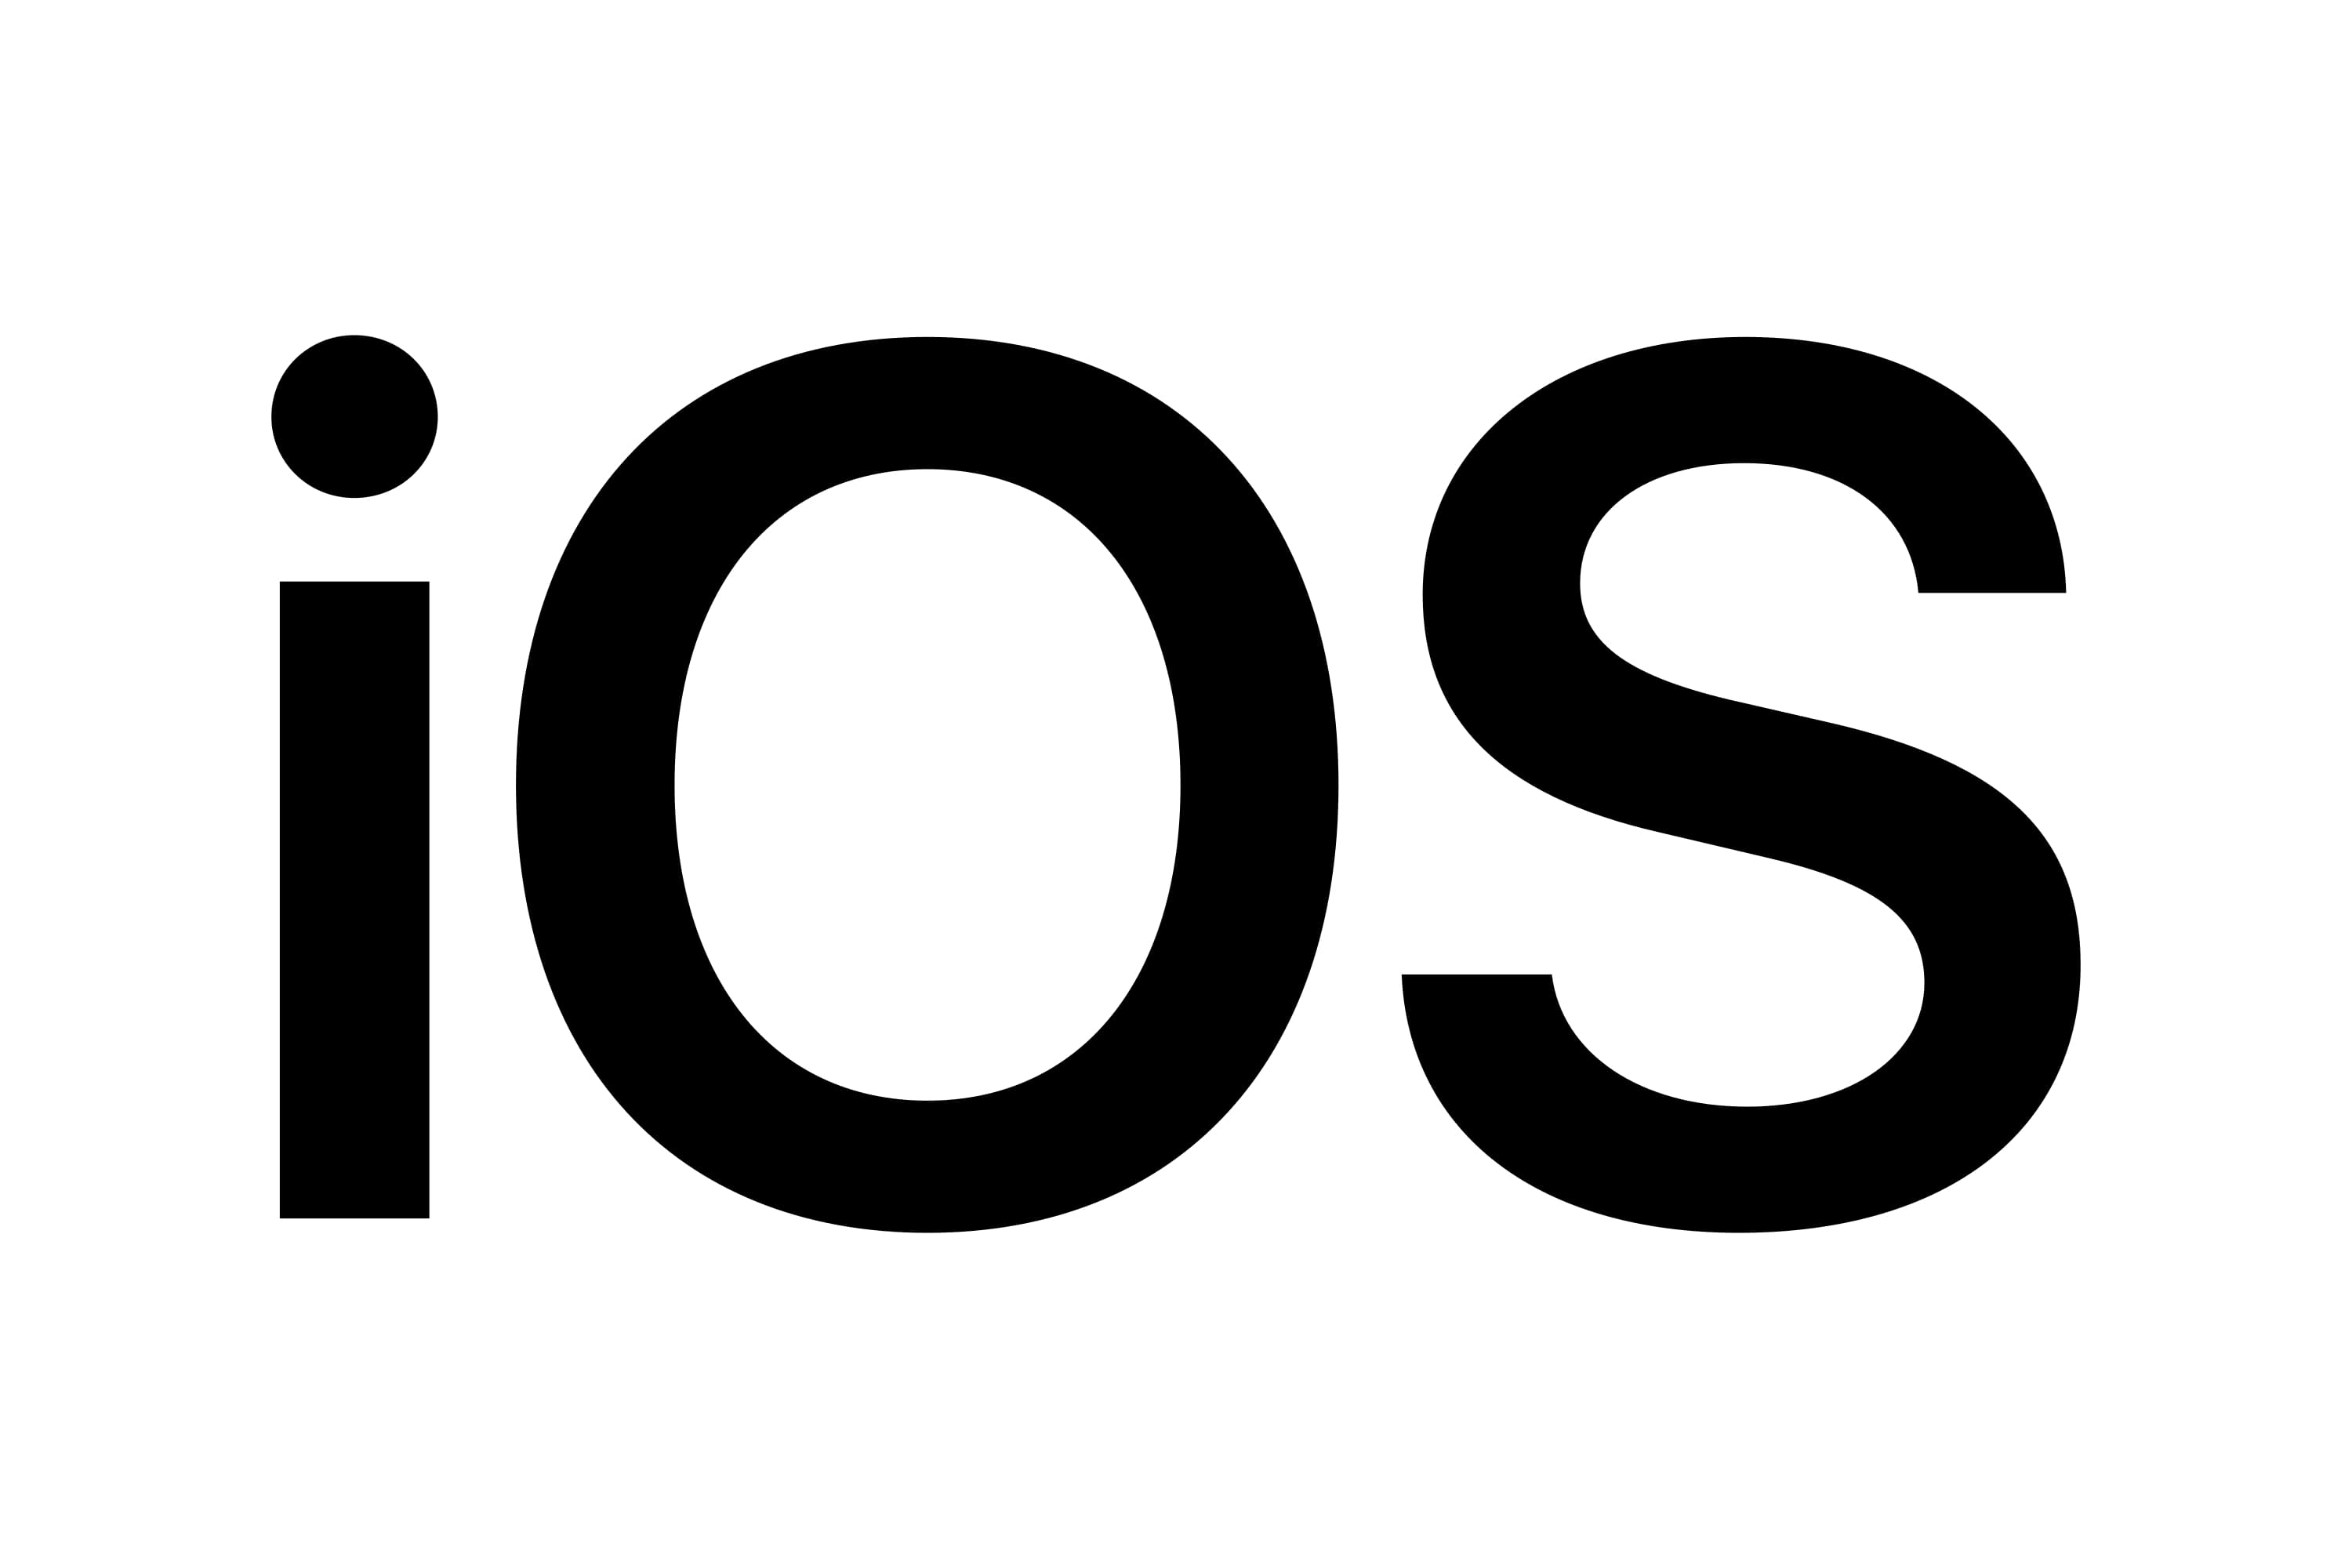
\includegraphics[width=1cm]{immagini/logoios.jpg}
 	\caption{Logo iOS}
 	\label{fig:Logo iOS}
 \end{figure}
 iOS è il sistema operativo sviluppato da Apple per dispositivi iPhone, iPod touch e iPad.\\
 Per un lungo periodo il linguaggio per sviluppare un'applicazione iOS è stato Objective-C che deriva da C e C++. \\
 Per aumentare la produttività, Apple ha lanciato un linguaggio di più alto livello ovvero Swift. Swift è veloce, leggibile e poco prolisso. Nonostante ciò, Objective-C viene ancora preferito quando si sta lavorando più a basso livello.\\

 \subsubsection{Windows Phone}
 \begin{figure}[htbp]	
 	\centering
 	
\includegraphics[width=3cm]{immagini/logowindowsphone.png}
 	\caption{Logo Windows Phone}
 	\label{fig:Logo Windows Phone}
 \end{figure}
Windows Phone è il sistema operativo sviluppato da Microsoft.\\
Il linguaggio utilizzato per sviluppare un'applicazione Windows Phone è C\#, che è un linguaggio semi-compilato orientato agli oggetti.\\
Con Android e iOS in ambito mobile non c'è paragone. Invece per quanto riguarda sistemi desktop, Windows risulta una delle migliori.\\
 
\subsection{Web app}
Una web app \cite{differenza,apptonative} è un'applicazione che funziona come un sito web adattandosi al dispositivo utilizzato.\\
Queste applicazioni non necessitano di essere installate sugli smartphone e quindi non andranno ad aumentare la memoria utilizzata nel dispositivo.\\
 Inoltre non possono essere pubblicate sugli Store e quindi non godono di un enorme visibilità.\\
I principali framework e librerie per creare una web app sono:
\begin{itemize}
	\item Angular; 
	\item PolymerJS; 
	\item React.
\end{itemize}
I vantaggi di sviluppare una web app sono:
\begin{itemize}
	\item Scrittura con Markup HTML;
	\item Non essendo pubblicate sul Market non devono essere sottoposte al processo di approvazione; 
	\item Minor tempo di sviluppo.
\end{itemize}

\newpage

\subsection{App Ibride Web View Wrapper}
Questo tipo di metodo \cite{differenza,apptonative} permette di creare applicazioni senza alcuna conversione del codice in base al sistema operativo.\\
 In pratica l'applicazione rileva inizialmente il sistema operativo utilizzato e successivamente imita l'aspetto dell'interfaccia utente, utilizzando CSS, Sass...\\
Le piattaforme più usate sono:
\begin{itemize}
\item Ionic; 
\item Apache Cordova; 
\item PhoneGap.
\end{itemize}
I vantaggi principali di Ionic e delle App Ibride Web View Wrapper sono:
\begin{itemize}
	\item Riutilizzo facile del codice; 
	\item Ionic utilizza JavaScript e fornisce un supporto per Angular;
	\item Addatamento automatico in base alla piattaforma; 
\end{itemize}
Lo svantaggio principale di questo tipo di applicazioni sta in termini di velocità di calcolo e questo comporterà prestazioni inferiori alle applicazione compilate in nativo.\\

\subsection{App Ibride Compile to Native}
Le applicazioni ibride che compilano in nativo utilizzano un unico linguaggio di programmazione per la scrittura del codice. Una volta compilato i componenti dell'interfaccia utente del codice vengono convertiti nei componenti dell'interfaccia utente nativi senza bisogno di configurazioni particolari.\\
Le principali piattaforme utilizzate per compilare in nativo sono:
\begin{itemize}
	\item React Native; 
	\item NativeScript; 
	\item Xamarin; 
	\item Flutter.
\end{itemize}
I vantaggi principali di utilizzare piattaforme che compilano in nativo sono:
\begin{itemize}
	\item Anche se minore delle App Ibride Web View Wrapper hanno un elevata riutilizzabilità del codice; 
	\item Elevato numero di librerie utilizzabili;  
	\item Compilando in nativo offrono prestazioni elevate.
\end{itemize}
\newpage
\section{Flutter}
\begin{figure}[htbp]	
	\centering
	
\includegraphics[width=6cm]{immagini/flutterlogo.jpg}
	\caption{Logo Flutter}
	\label{fig:Logo Flutter}
\end{figure}
Flutter \cite{flutterprogramma} è un framework nato abbastanza di recente per lo sviluppo di applicazioni per diverse piattaforme.\\
È stato ideato da Google come progetto open source e pubblicato ufficialmente per la prima volta a dicembre del 2018 nella versione 1.0 all'evento Flutter Live.\\
Il 3 marzo 2021 è stata rilasciata la versione 2.0 che consente agli sviluppatori di generare in maniera stabile applicazioni multipiattaforma.\\
Flutter offre una vasta serie di librerie di elementi di interfaccia utente e combina la facilità di sviluppo con prestazioni simili alle prestazioni native, mantenendo una corretta distinzione visiva tra le diverse piattaforme senza che il programmatore debba prestare particolari attenzioni.
Viene utilizzato sopratutto per applicazione Android e iOS e funziona come una vera applicazione nativa.\\
Utilizzando lo stesso codebase è possibile creare l'applicazione per diverse piattaforme.\\
Il linguaggio di programmazione di Flutter è Dart, sviluppato anche esso da Google, ed è stato pensato per sostituire JavaScript.\\
Flutter è completamente gratuito e come possiamo vedere dalla figura sottostante, già nell'ultimo anno la sua popolarità e utilizzo è cresciuta notevolmente.\\
\begin{figure}[htbp]	
	\centering
	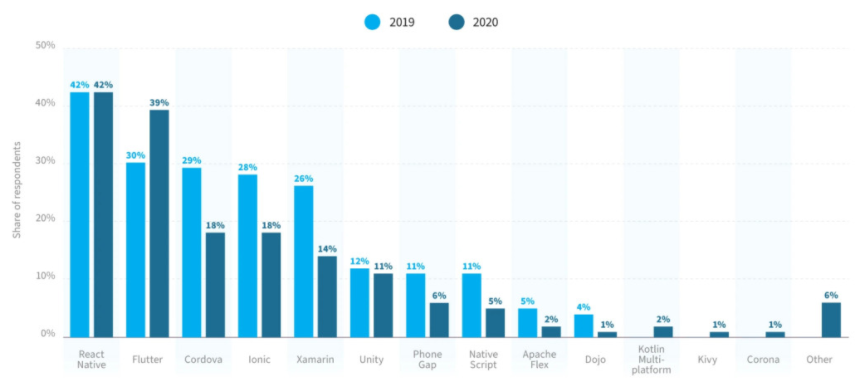
\includegraphics[width=13cm]{immagini/statisticheflutter.png}
	\caption{Statistiche dei programmatori che usano Flutter per sviluppare app mobile}
	\label{fig:Statistiche dei programmatori che usano Flutter per sviluppare app mobile}
\end{figure}
\newpage
Anche se molto recente, nel Google Play Store possiamo contare oltre 50000 applicazioni Flutter.\\
I vantaggi di utilizzare Flutter sono:
\begin{itemize}
	\item Un codebase per tutte le piattaforme; 
	\item Utilizzo di \hyperref[sec:Dart]{Dart} che è un linguaggio facile da apprendere;  
	\item Più facile da sviluppare applicazioni con Flutter che quindi entrano sul mercato più in fretta;
	\item Si basa sul principio \textit{'Tutto è un Widget'} che sarà spiegato nella \hyperref[sec:Widget]{sezione Widget};
	\item Basso consumo di risorse;
	\item Esecuzione performante delle app native su smartphone;
	\item Ottima interfaccia utente che può essere anche personalizzata;
	\item L’hot reload permette di vedere le modifiche in tempo reale accelerando lo sviluppo.\\
\end{itemize}
Invece tra gli svantaggi possiamo citare che:
\begin{itemize}
	\item Dart è un linguaggio nuovo e quindi non molto diffuso; 
	\item Essendo nuovo mancano librerie di terze parti che facilitano lo sviluppo;  
	\item Vengono create app di grandi dimensioni rispetto agli altri framework o anche a Java stesso.\\
\end{itemize}
\subsection{Dart}
\label{sec:Dart}
Dart \cite{dart,dartstoria} è un linguaggio di programmazione sviluppato da Google e presentato per la prima volta il 10 ottobre del 2011 alla conferenza 'GOTO Aarhus 2011'.\\
Lo scopo principale è quello di sostituire JavaScript per lo sviluppo delle applicazioni.\\
Dart costituisce la base di Flutter e inoltre supporta molte attività di sviluppo di base come la formattazione, l'analisi, il test del codice...\\
Dart è type-safe. Inoltre i valori in Dart non possono essere null tranne nei casi in cui viene indicato che questi valori possono esserlo, così da evitare possibili errori nel codice.\\
Dart ha un vasto numero di librerie di base e di pacchetti per le API aggiuntive.\\
Dart permette di scrivere programmi attraverso due distinte piattaforme:
\begin{itemize}
	\item Dart Native: per le applicazioni sviluppate per dispositivi mobili e desktop. Include sia una macchina virtuale Dart con compilazione JIT (just-in-time), ovvero viene compilato durante l'esecuzione del programma, sia un compilatore AOT (Ahead-of-Time) per la produzione di codice macchina, ovvero  viene compilato prima dell'esecuzione, tipicamente durante l'installazione del programma così migliorando le prestazioni evitando la fase di compilazione durante l'esecuzione del programma;  
	\item Dart Web: per le applicazioni destinate al Web. Include sia un compilatore del tempo di sviluppo (dartdevc) che consente di eseguire il debug dell'applicazione nel browser Chrome e vedere le modifiche quasi immediatamente, che un compilatore del tempo di produzione (dart2js) che fornisce suggerimenti per migliorare il codice Dart e rimuovere il codice inutilizzato. Entrambi i compilatori traducono Dart in JavaScript.\\
\end{itemize}

\subsection{Componenti}
Flutter è formato da un'architettura a strati e i suoi tre strati fondamentali sono:
\begin{itemize}
	\item Framework; 
	\item Engine;  
	\item Embedder.\\
\end{itemize}
\begin{figure}[htbp]	
	\centering
	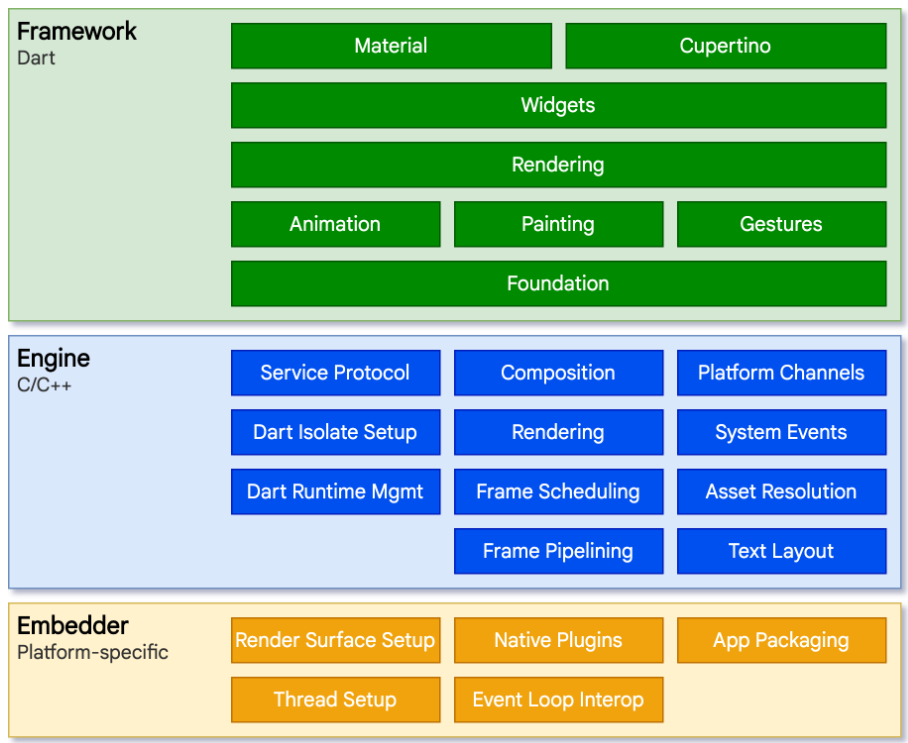
\includegraphics[width=13cm]{immagini/composizione.png}
	\caption{Architettura a strati di Flutter}
	\label{fig:Architettura a strati di Flutter}
\end{figure}

\newpage

\subsubsection{Embedder}
Embedder è il livello più basso dell'architettura.\\
Il linguaggio utilizzato è definito in base alla piattaforma e attualmente può essere: Java e C++ per Android, Objective-C/Objective-C++ per iOS e macOS e C++ per Windows e Linux.
Ha lo scopo di legare il rendering della schermata nativa, la gestione degli eventi,...\\
Per fare ciò lo strato Embedder interagisce con lo strato Engine tramite delle API C/C++.
Inoltre lo strato Embedder è composta da una Shell che ospita anche la Dart VM.		\\
Ogni Shell è specifica per ogni piattaforma e offre un accesso alle API native della piattaforma in questione.

\subsubsection{Engine}
Engine è lo strato intermedio dell'architettura.\\
Il linguaggio utilizzato è principalmente il C++ e il C per rendere più veloci ed efficienti le applicazioni realizzate in Flutter.\\
Contiene componenti di basso livello essenziali per il funzionamento del framework.\\
All'interno troviamo il motore grafico \textit{Skia}, una libreria grafica 2D open source scritta in C++ creata da Google, e le shell a cui è possibile accedervi tramite le API esposte dalla libreria \textit{dart:ui}.

\subsubsection{Framework}
È lo strato principale dell'architettura.\\
Il linguaggio utilizzato è \hyperref[sec:Dart]{Dart}.\\
All'interno sono presenti classi fondamentali di base e servizi di base come l'animazione.\\
Inoltre è presente il Rendering che permette di gestire il layout attraverso un albero di oggetti che viene visualizzato
a schermo e che si aggiorna automaticamente.\\
Sempre all'interno di questo strato sono presenti i Widgets e le due librerie: Material e Cupertino.

\newpage

\subsection{Librerie Material e Cupertino}
Le due principali librerie di Flutter sono Material e Cupertino.\\
\begin{figure}[htbp]	
	\centering
	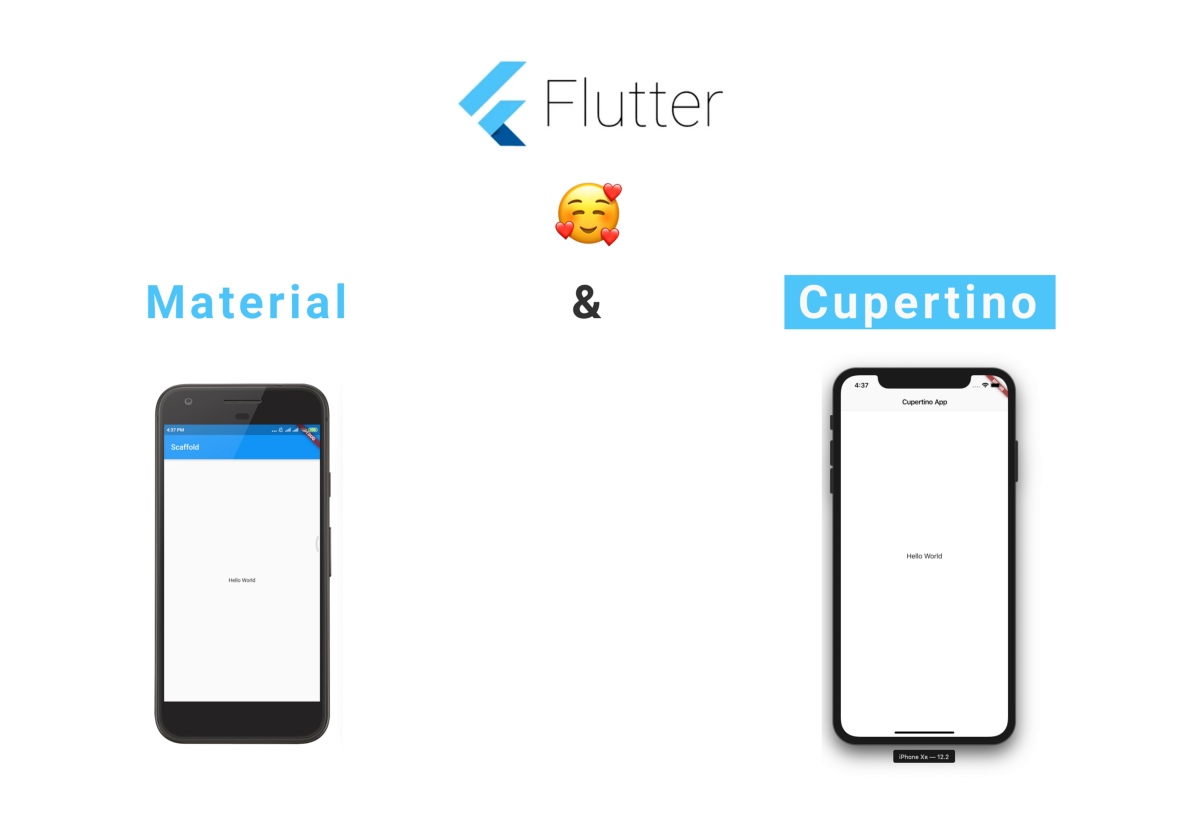
\includegraphics[width=14cm]{immagini/librerieCM.png}
	\caption{Librerie Material e Cupertino}
	\label{fig:Librerie Material e Cupertino}
\end{figure}
\\
All'interno di Flutter è possibile capire su che piattaforma si sta eseguendo l'applicazione attraverso \textit{'Platform.isIOS'}. Se ritornerà \textit{true} significa che saremo su iOS altrimenti saremo su Android.\\
La libreria Cupertino permette di implementare un design specifico per le applicazioni iOS.\\
A differenza della Cupertino la libreria Material permette di implementare un design specifico per le applicazioni Android.

\subsection{Widget}
\label{sec:Widget}
Flutter è basato sul principio \textit{'Tutto è un widget'} in quanto l'interfaccia di un programma è composta da diversi widget nidificati.\\
Ogni widget può essere testo o un pulsante o qualsiasi altro elemento grafico che contiene varie caratteristiche. Tutti questi widget possono influenzare altri widget nella costruzione dell'applicazione.\\
Il vantaggio principale di questa struttura a widget consiste nella flessibilità, invece lo svantaggio di adottare questa strategia sta nel fatto che tutti i widget sono situati nel codice sorgente del programma e pertanto risulteranno fortemente nidificati.
\newpage
Il framework contiene due classi principali di widget:
\begin{itemize}
	\item Stateless widget;   
	\item Stateful widget.
\end{itemize}
\cite{state}

\begin{figure}[htbp]	
	\centering
	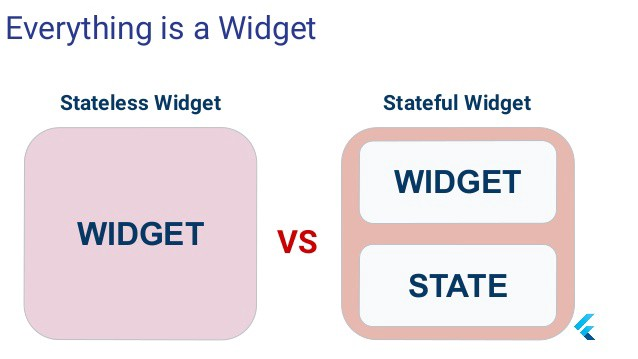
\includegraphics[width=13cm]{immagini/state.jpeg}
	\caption{Stateless widget e Stateful widget}
	\label{fig:Stateless widget e Stateful widget}
\end{figure}
\subsubsection{Stateless widget}
Gli stateless widget non hanno uno stato mutabile e quindi non cambieranno nel tempo neanche in seguito a comportamenti effettuati dall'utente.\\
Alcuni esempi di questi widget sono: Text, Row, Column e Container.\\
Per creare uno stateless widger bisogna estendere la classe \textit{SteatelessWidget} che richiedere l'override del metodo \textit{build()}.\\
Questo metodo viene invocato la prima volta per costruire l'albero dei widget e quando le loro dipendenze cambiano.\\
Si puo usare uno stateless widget solamente quando i campi dei widget non cambiano nel tempo neanche dopo azioni dell'utente.
Negli altri casi sarà da utilizzare uno stateful widget.

\subsubsection{Stateful widget}
Gli stateful widget sono dinamici e mutano nel tempio in base all'interazione dell'utente o in base ad altri fattori.\\
Alcuni esempi di questi widget sono: Iamge, Form e Checkbox.\\
Per creare uno stateful widger bisogna estendere la classe \textit{SteatefulWidget}.\\
Dipende dallo stato dell'oggetto. Infatti ogni volta che si vuole modificare lo stato di un qualsiasi oggetto bisogna chiamare il metodo \textit{setState()} segnalando così al framework di aggiornare l'interfaccia utente chiamando il metodo build e tenendo in considerazione i nuovi stati degli oggetti segnalati nel metodo appena descritto. \\
Possiamo quindi creare uno stateful widget quando il widget potrebbe cambiare durante il suo ciclo di vita. 

\newpage

\subsubsection{Principali Widget}
Di seguito saranno spiegati brevemente i widget più comuni e utilizzati in Flutter.

\paragraph{Scaffold}
Scaffold \cite{scaffold} implementa la struttura del layout visivo.\\
Contiene principalmente 5 elementi:
\begin{itemize}
	\item \textbf{appBar} che viene descritta di seguito;   
	\item \textbf{body} che rappresenta il corpo situato sotto l'Appbar;
	\item \textbf{floatingActionButton} che è un bottone che è situato di default in basso a destra;   
	\item \textbf{drawer} che è un menù laterale visibile dall'utente scorrendo da sinistra a destra o viceversa. All'interno di questo menù sono presenti altri widget che permettono di effettuare diverse azioni;
	\item \textbf{bottomNavigationBar} che permette di gestire un menù nella parte inferiore dell'applicazione.
\end{itemize}

\begin{figure}[htbp]	
	\centering
	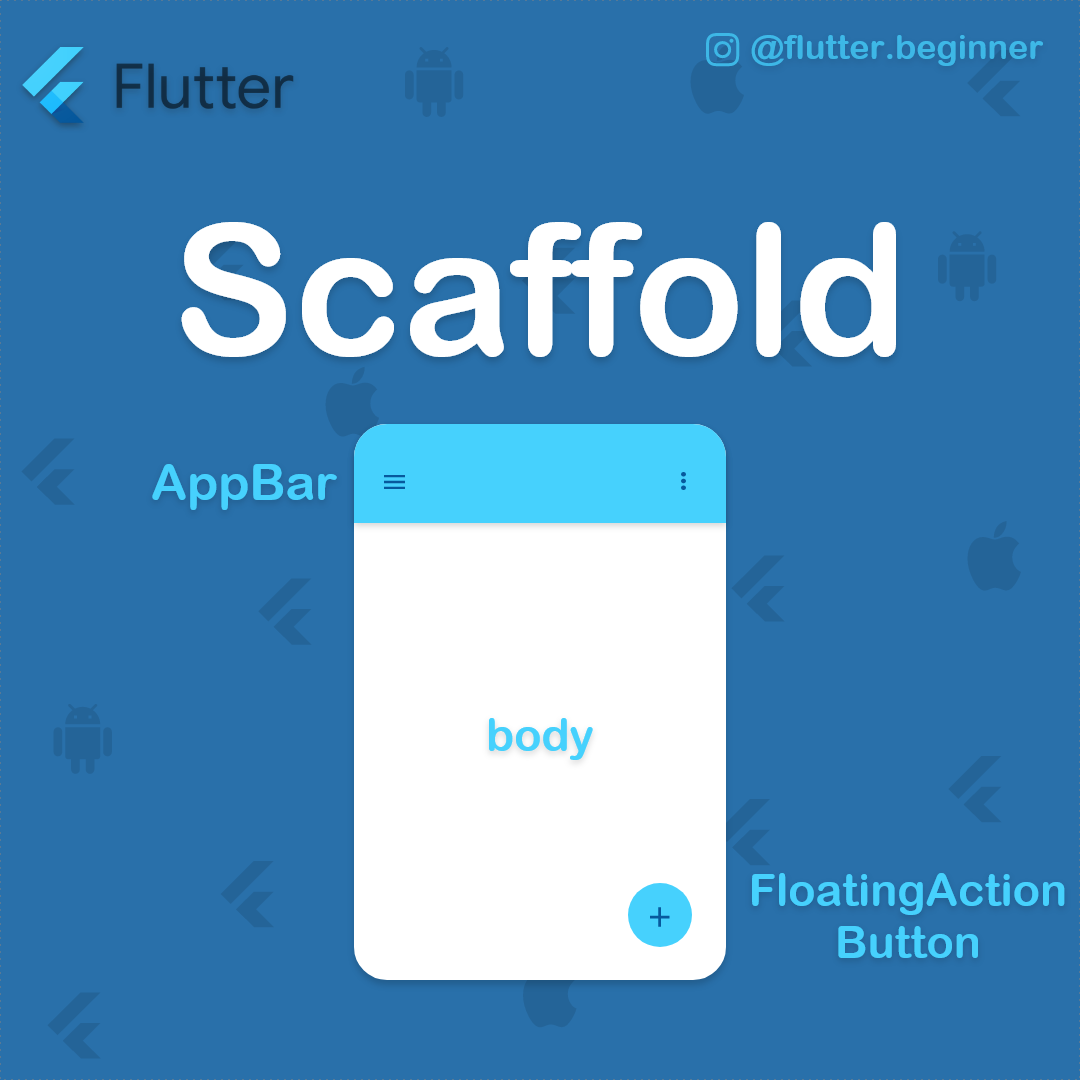
\includegraphics[width=8cm]{immagini/scaffold.png}
	\caption{Scaffold widget}
	\label{fig:Scaffold widget}
\end{figure}

\newpage

\paragraph{AppBar}
L'AppBar viene gestita da Scaffold ed è solitamente situata nella parte superiore dell'applicazione e espone solitamente anche altri widget che permettono di eseguire una o più azioni.\\
AppBar ha diverse elementi grafici come elevazione e titolo.
\begin{figure}[htbp]	
	\centering
	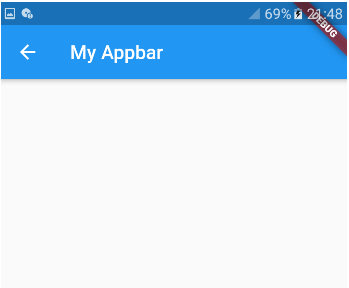
\includegraphics[width=8cm]{immagini/appbar.png}
	\caption{Appbar widget}
	\label{fig:Appbar widget}
\end{figure}

\paragraph{Row, Column}
Il widget Row permette di creare una famiglia di widget in una riga orizzontale invece il widget Column permette di creare sempre una famiglia di widget ma in verticale.\\
Entrambi non sono scorrevoli quindi nel caso si abbia bisogno di una famiglia di widget scorrevoli bisogna utilizzare il widget \textit{ListView}.
\begin{figure}[htbp]	
	\centering
	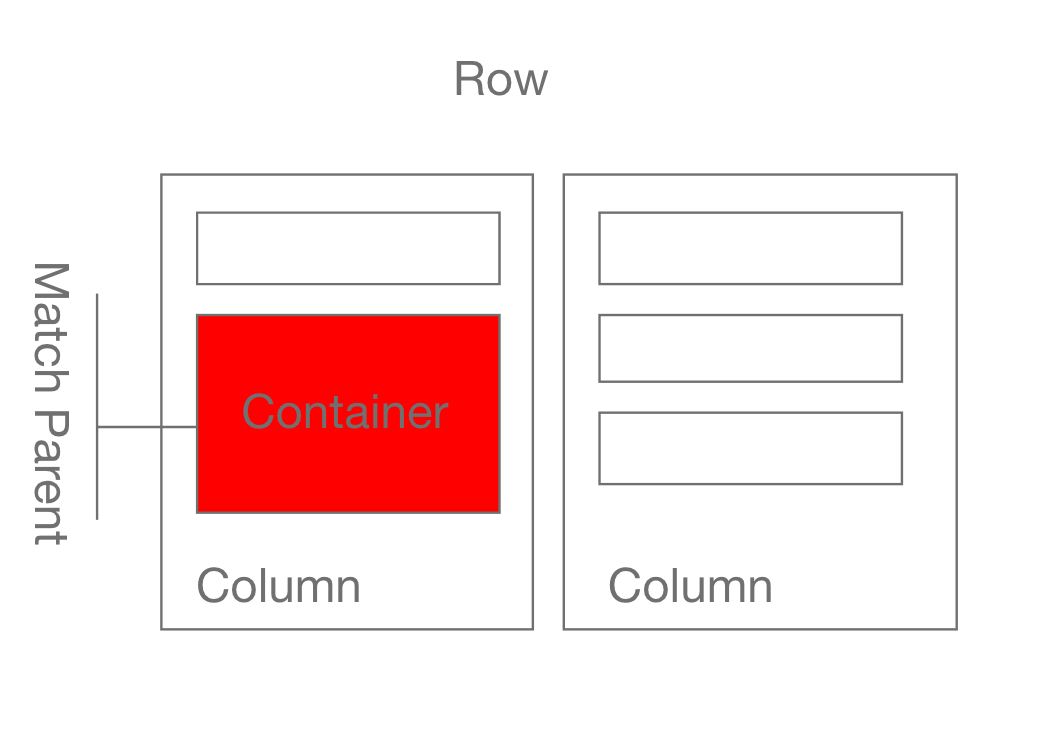
\includegraphics[width=10cm]{immagini/rowcolumn.png}
	\caption{Row e Column widgets}
	\label{fig:Row e Column widgets}
\end{figure}

\newpage

\paragraph{Container}
Il widget Container funge da contenitore all'interno dell'applicazione e può racchiudere altri widget.\\
Ha un margine, un bordo e un padding di default che possono essere modificati.\\
Oltre a questi elementi questo widget contiene altri elementi che permettono di decorare la sua area di competenza.
\begin{figure}[htbp]	
	\centering
	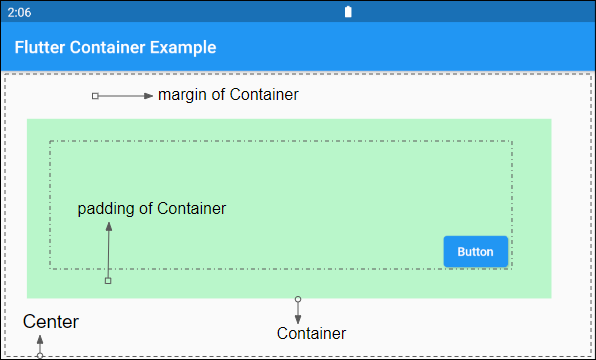
\includegraphics[width=8cm]{immagini/container.png}
	\caption{Container widget}
	\label{fig:Container widget}
\end{figure}

\paragraph{Text}
Il widget Text consente di creare una porzione di testo all'interno dell'applicazione che può essere decorata in base alle diverse esigenze.
\begin{figure}[htbp]	
	\centering
	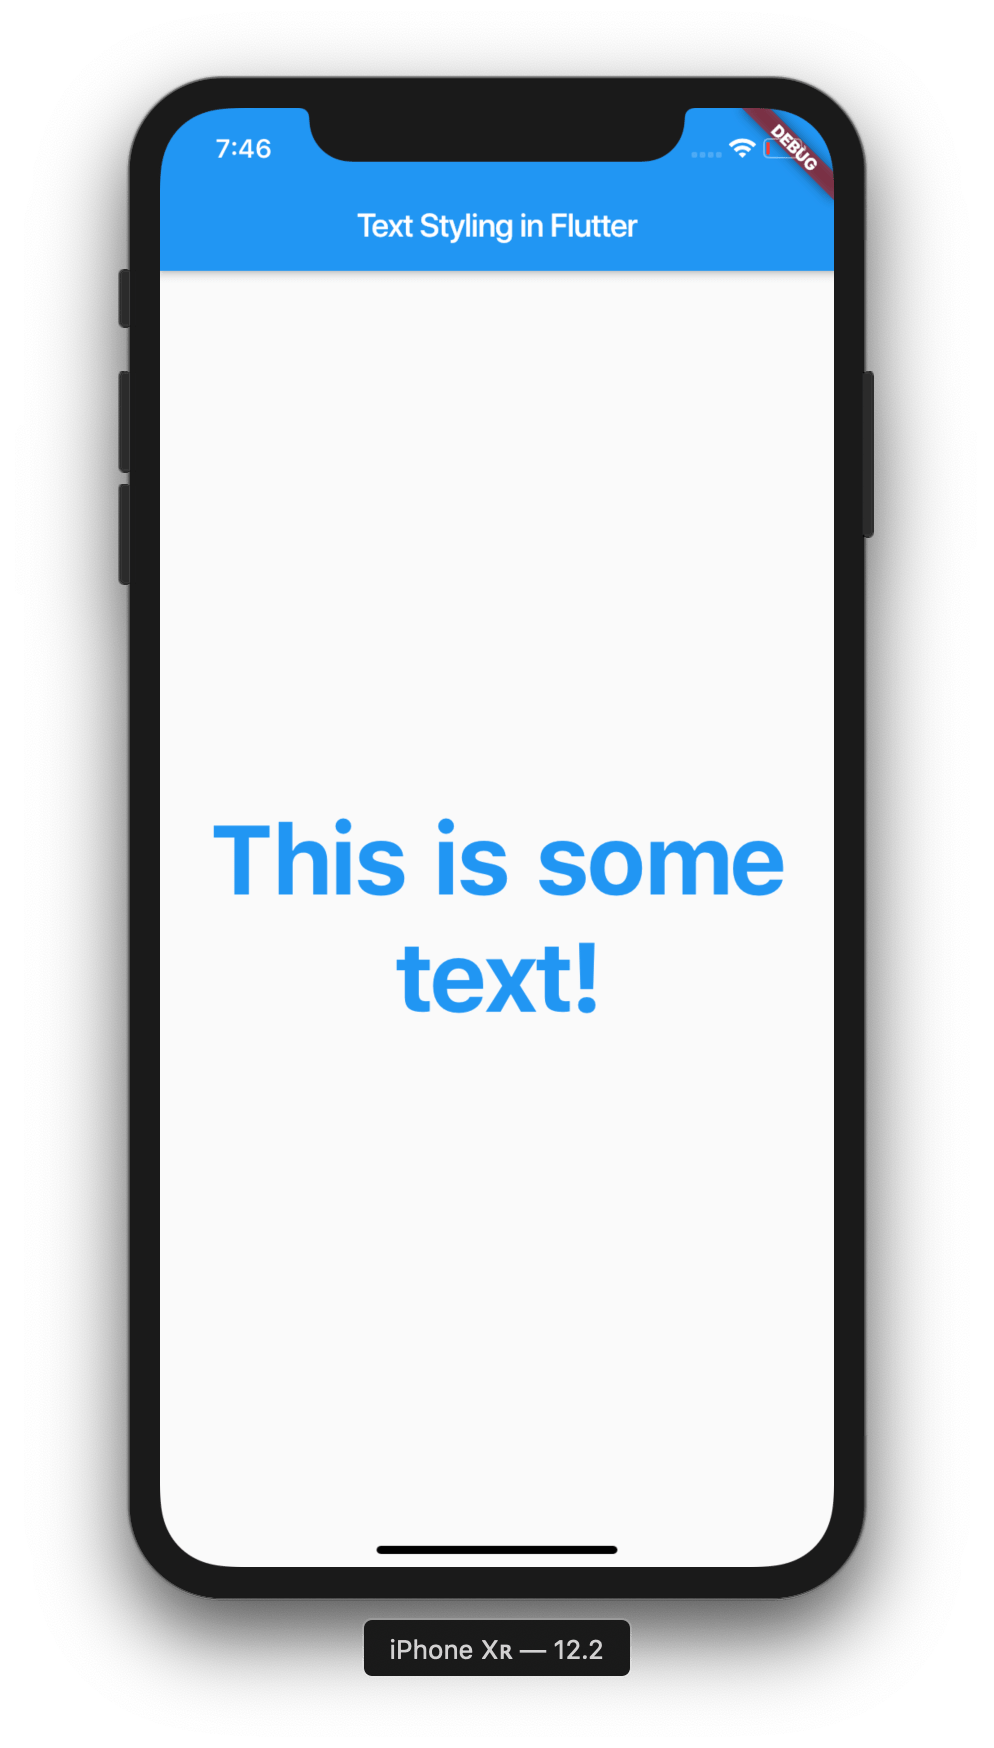
\includegraphics[width=5cm]{immagini/text.png}
	\caption{Text widget}
	\label{fig:Text widget}
\end{figure}

\paragraph{Image}
Consente di apportare all'interno dell'applicazione un'immagine.\\
Ci sono vari formati disponibili ovvero JPEG, PNG, GIF.\\
I modi per ottenere l'immagine all'interno dell'applicazione sono:
\begin{itemize}
	\item \textbf{new Image} che permette di ottenere un'immagine da un  ImageProvider(utilizza imageCache globale per memorizzare nella cache le immagini);   
	\item \textbf{new Image.asset} che permette di ottenere un'immagine da un AssetBundle(una raccolta di risorse utilizzate dall'applicazione) utilizzando una chiave;
	\item \textbf{new Image.network} che permette di ottenere un'immagine da un URL;   
	\item \textbf{new Image.file} che permette di ottenere un'immagine da un File;
	\item \textbf{new Image.memory} che permette di ottenere un'immagine da un Uint8List.
\end{itemize}

\paragraph{Icon}
Il widget Icon permette di inserire icone all'interno dell'applicazione.\\
Le icone sono quadrate e non sono interattive.
\begin{figure}[htbp]	
	\centering
	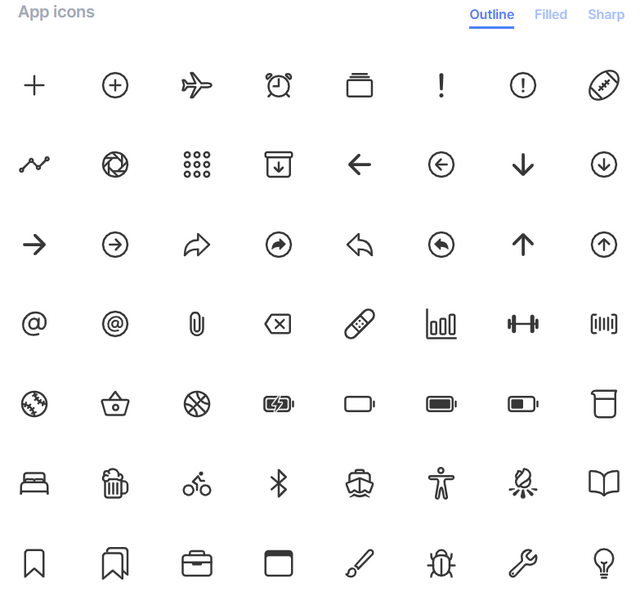
\includegraphics[width=5cm]{immagini/icon.png}
	\caption{Icon widget}
	\label{fig:Icon widget}
\end{figure}

\paragraph{ElevatedButton}
Il widget ElevatedButton permette di inserire un bottone con uno stile di default all'interno dell'applicazione.\\
Contiene l'elemento \textit{onPressed} che permette di eseguire operazioni quando il bottone sarà premuto. Nel caso onPressed sia uguale a null il bottone sarà disabilitato.
\begin{figure}[htbp]	
	\centering
	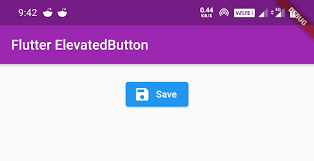
\includegraphics[width=8cm]{immagini/button.png}
	\caption{ElevatedButton widget}
	\label{fig:ElevatedButton widget}
\end{figure}

\newpage

\subsection{Esempi piccole applicazioni realizzate}
Di seguito verranno mostrate alcune applicazioni realizzate seguendo un corso su Udemy \cite{corso} per imparare a usare il framework Flutter.

\subsubsection{Applicazione base}
Dopo aver effettuato la giusta configurazione e scaricato tutto il necessario, per creare la prima applicazione di base messa a disposizione da Flutter basterà digitare sul terminale il comando: \textit{flutter create "nome\_applicazione"}.\\
Questo ci permette di creare la nostra prima applicazione base come esposto nella figura sottostante.\\

\begin{figure}[htbp]	
	\centering
	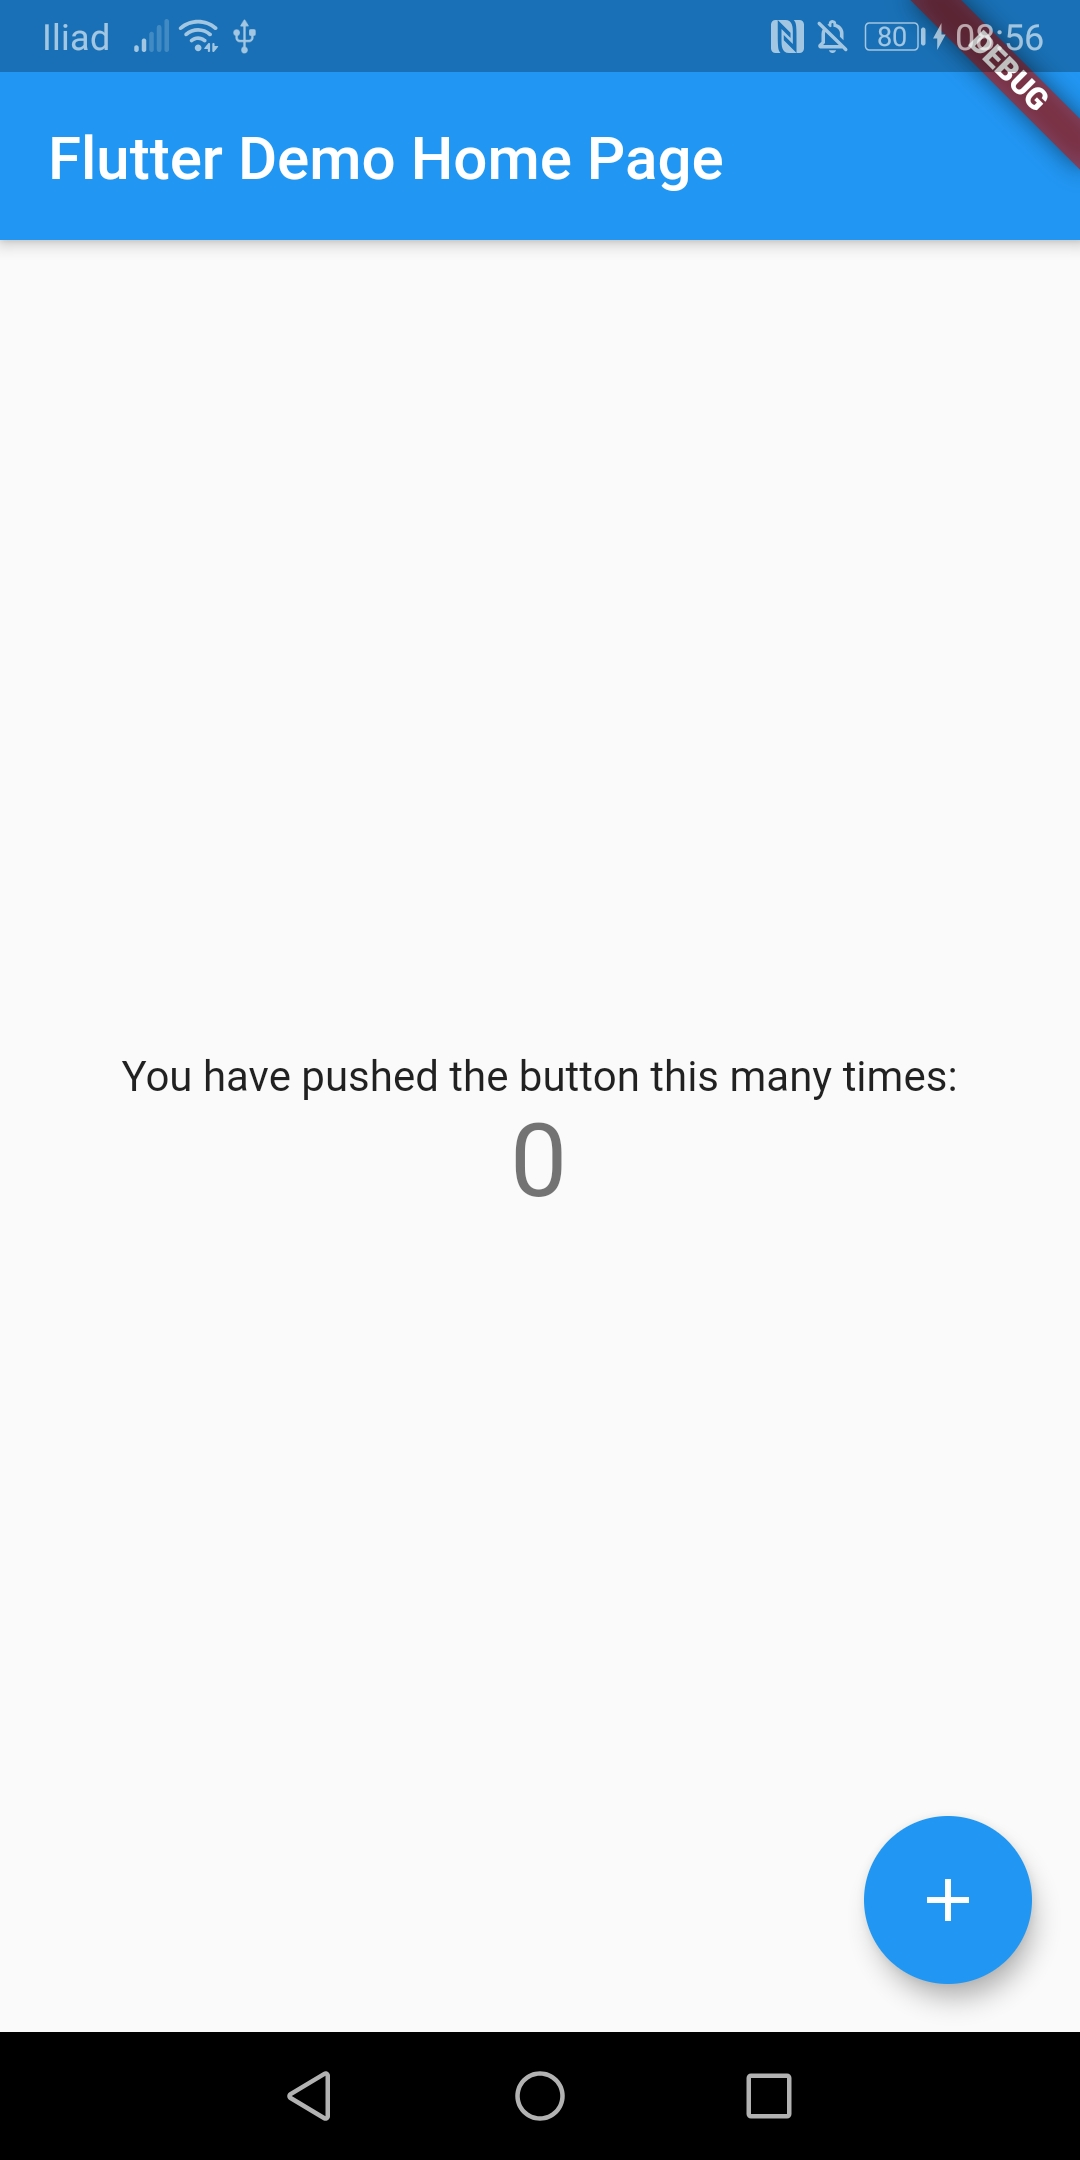
\includegraphics[width=6cm]{immagini/base.jpeg}
	\caption{Applicazione base}
	\label{fig:Applicazione base}
\end{figure}

\newpage

\subsubsection{Applicazione 1}
Questa applicazione permette di rispondere a una serie di domande e successivamente in base a un punteggio assegnato alla risposta selezionata da un giudizio finale.\\
Una volta terminato, il quiz può essere ritentato.\\
In particolare la creazione di questa applicazione mi ha permesso di apprendere meglio il funzionamento di alcuni widget fondamentali.\\
Tra questi sono stati visti principalmente i seguenti: AppBar, Text, Container, ElevatedButton.\\
Inoltre mi ha permesso anche di capire meglio gli attributi dei widget precedentemente elencati e mi ha fatto comprendere il funzionamento dello \textit{setState()}.\\

\begin{figure}[htbp]	
	\centering
	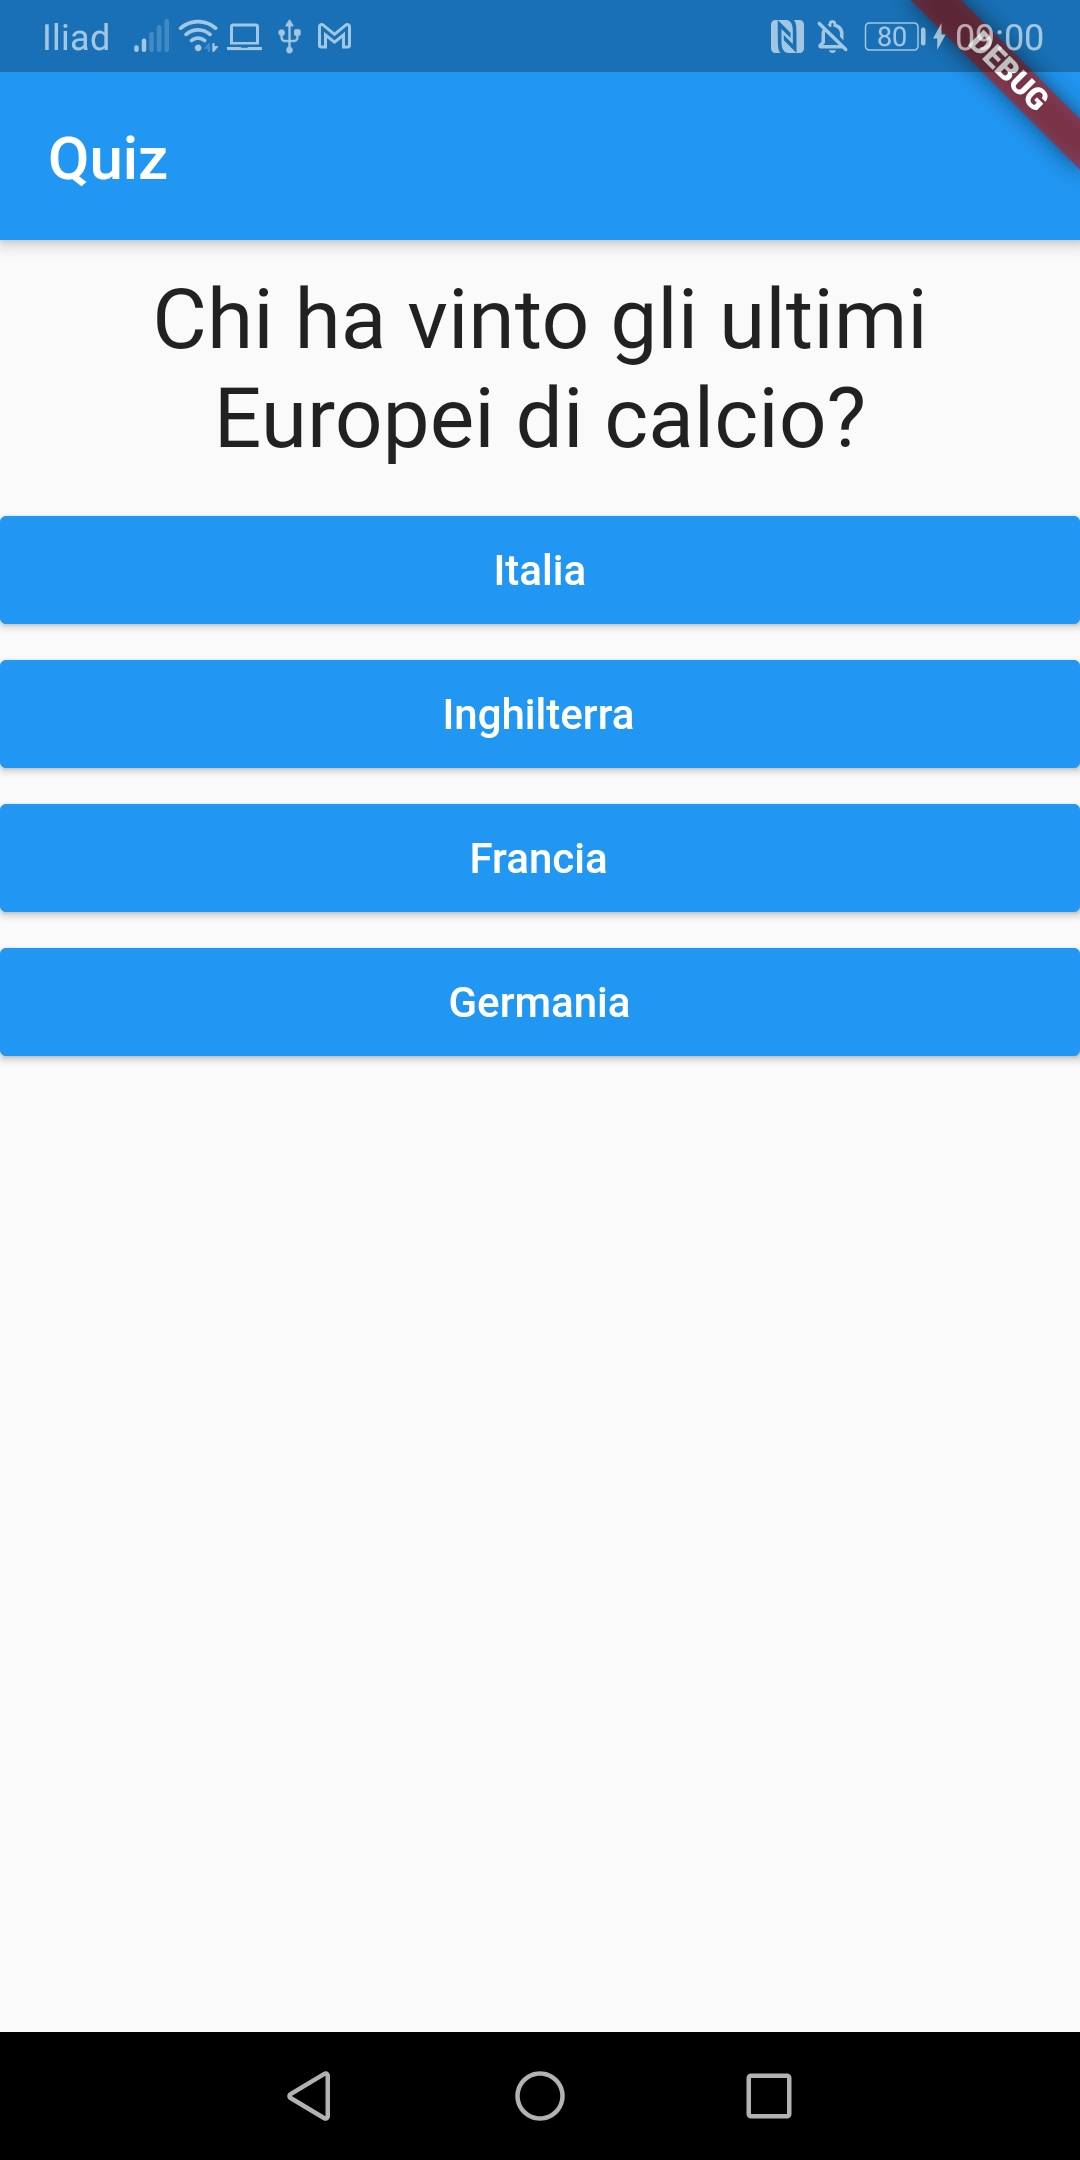
\includegraphics[width=6cm]{immagini/app1.jpeg}
	\caption{Applicazione 1}
	\label{fig:Applicazione 1}
\end{figure}

\newpage

\subsubsection{Applicazione 2}
Questa applicazione permette di inserire delle transizioni che un utente ha effettuato così da monitorare le spese sostenute.\\
In particolare mi ha permesso di comprendere alcuni attributi e widget più complessi rispetto a quelli base, studiare per bene il layout in modo che si adattasse alle dimensioni del cellulare, configurare una pagina in modo scrollabile e gestire widget a comparsa e scomparsa.\\

\begin{figure}[htbp]	
	\centering
	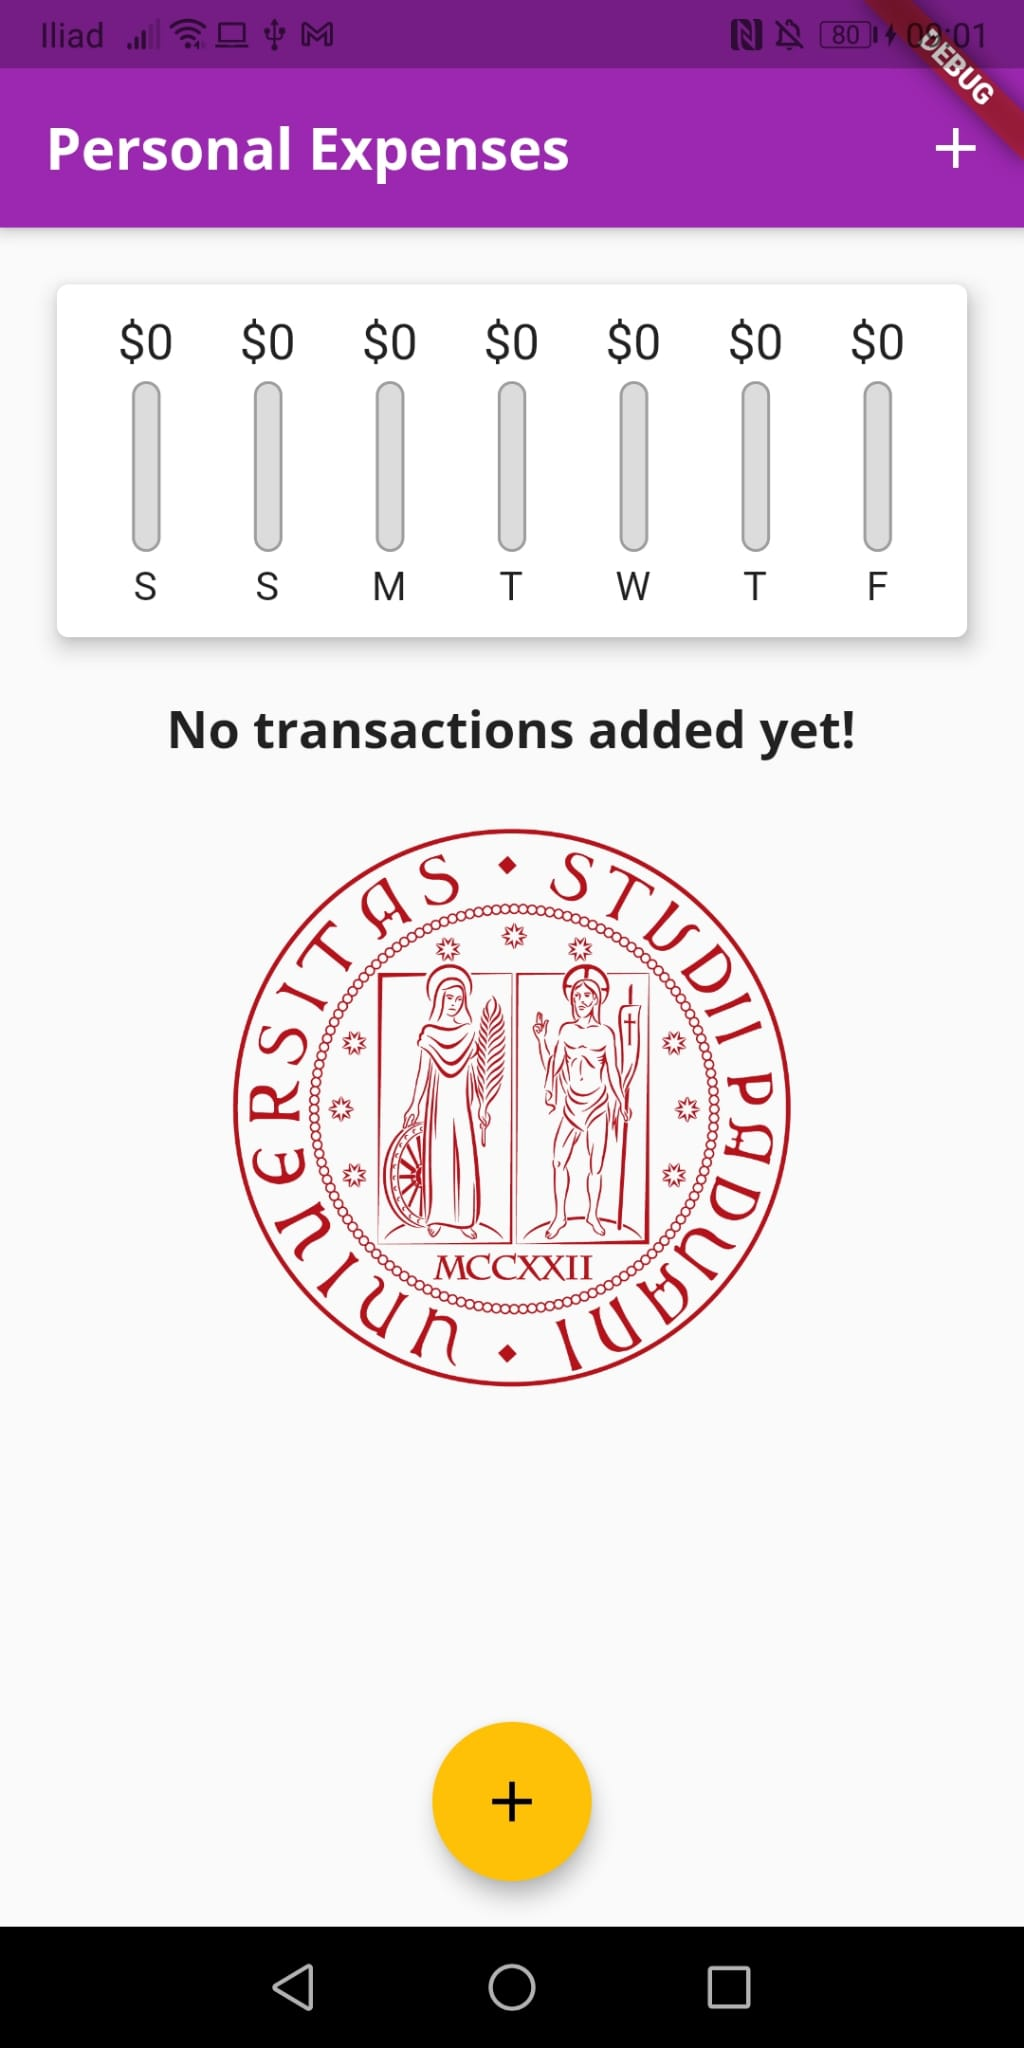
\includegraphics[width=6cm]{immagini/app2.jpeg}
	\caption{Applicazione 2}
	\label{fig:Applicazione 2}
\end{figure}

\newpage

\subsubsection{Applicazione 3}
Quest'ultima applicazione permette di gestire diverse categorie di cibi i quali contengono diverse ricette che possono essere aggiunte ai preferiti.\\
In particolare mi ha permesso di capire il corretto funzionamento delle Card, delle liste e come gestire nel menu laterale(drawer) i preferiti e i filtri.\\

\begin{figure}[htbp]	
	\centering
	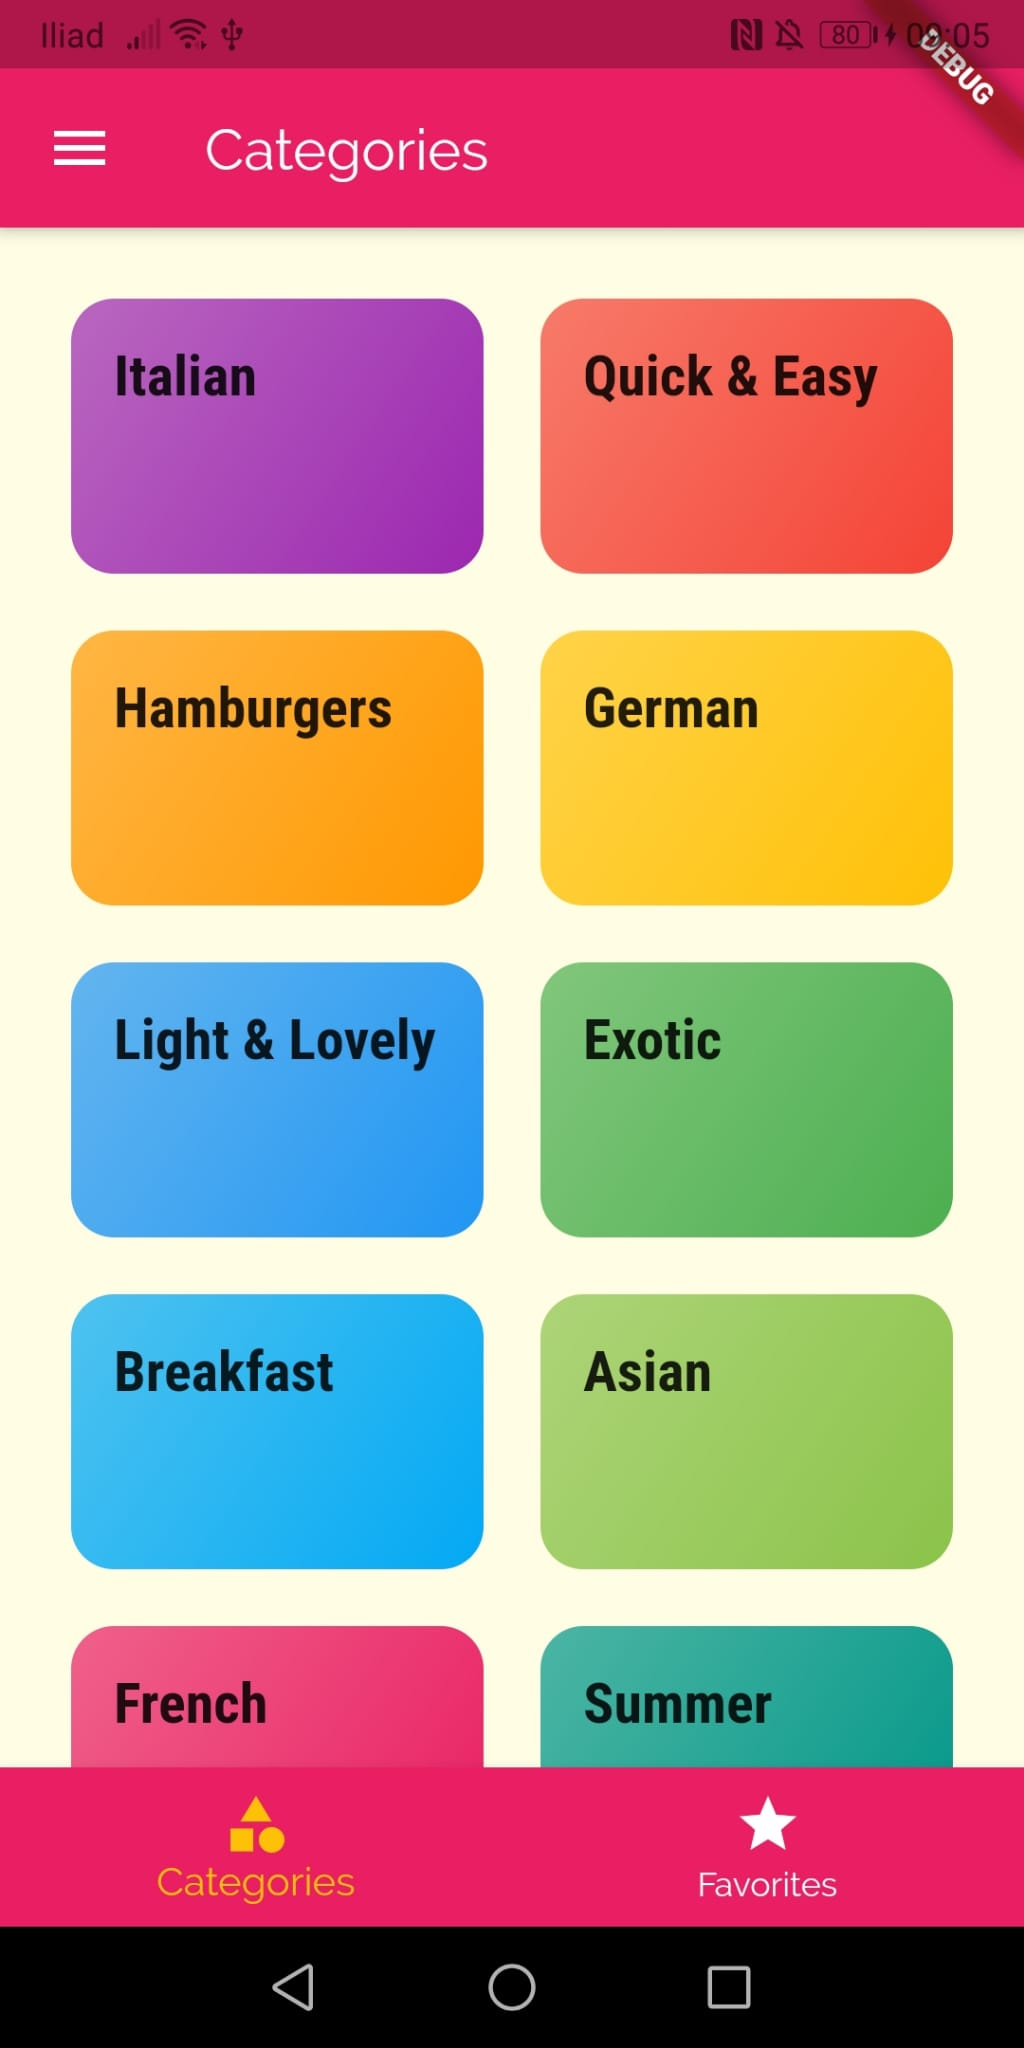
\includegraphics[width=6cm]{immagini/app3.jpeg}
	\caption{Applicazione 3}
	\label{fig:Applicazione 3}
\end{figure}






